\documentclass[a4paper,10pt]{article}
\usepackage[utf8]{inputenc}
\usepackage{amsmath}
\usepackage{caption}
\usepackage{graphicx}
\title{Lazy Caterer's Sequence}
\author{William Peters, Gihan Mendis}

\begin{document}

\maketitle

\section{Illustration of structures}

\subsection{Pancake Structure}
\begin{enumerate}
  \item $n = 4$\\
  	\begin{enumerate}
    	\item Pancake structure\\
    	\begin{figure}[h!]
			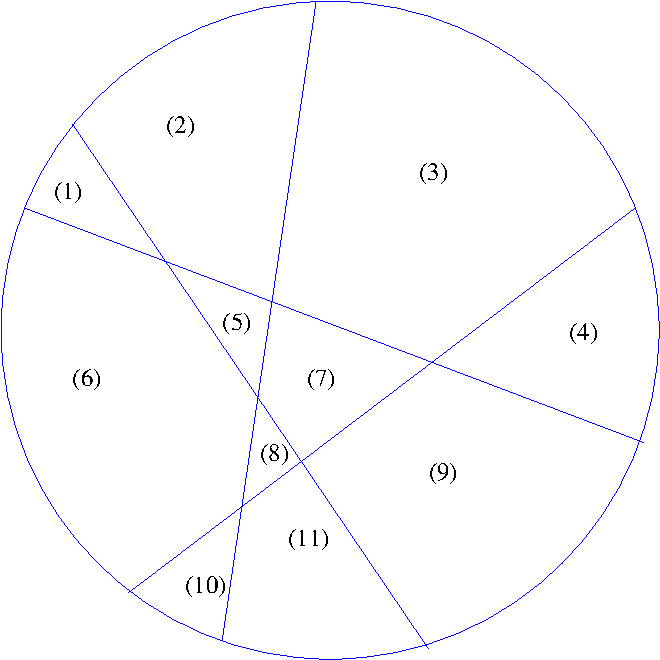
\includegraphics[scale=0.3]{graphics/pancakecut11}
			\captionsetup{labelformat=empty}
			\caption{}
			\label{fig:pancakecut11}
		\end{figure}
  \end{enumerate}
  
  %This should be n = 5 not 4 
  \item $n = 4$\\
  \begin{enumerate}
    \item Pancake structure\\
      \begin{figure}[h!]
			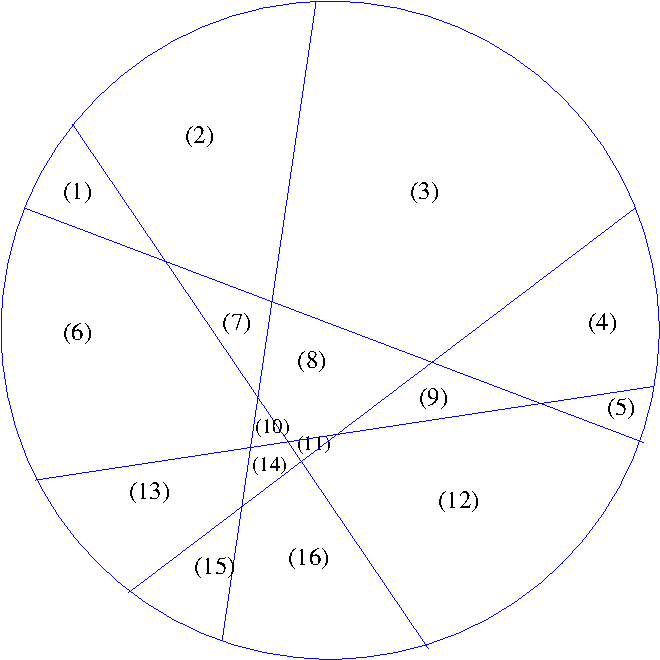
\includegraphics[scale=0.3]{graphics/pancakecut16}
			\captionsetup{labelformat=empty}
			\caption{}
			\label{fig:pancakecut16}
		\end{figure}
  \end{enumerate}
\end{enumerate}

\section{Formula Demonstrations}
\subsection{Binomial}
\begin{enumerate}
 \item $a(n) = Binomial(n+2,1)-2\times Binomial(n+1,1)+Binomial(n+2,2)$\\

  \hspace{1cm}${n+2 \choose 1} - 2\times {n+1 \choose 1} + {n+2 \choose 2}$\\
  \begin{enumerate}
    \item $n = 4$
    \[
     \boxed{ 
	  \begin{gathered}
       	a(4) = {4+2 \choose 1} - 2\times {4+1 \choose 1} + {4+2 \choose 2}\\
		\\ 
       	a(4) = {6 \choose 1} - 2\times {5 \choose 1} + {6 \choose 2} \\
       	\\
       	a(4) = 6 - 10 + 15\\
       	\\
       	a(4) = 11 
      \end{gathered}	    
	  }
    \]	  
    \item $ n = 5$
    \[
     \boxed{ 
	  \begin{gathered}
       	a(5) = {5+2 \choose 1} - 2\times {5+1 \choose 1} + {5+2 \choose 2}\\
		\\ 
       	a(5) = {7 \choose 1} - 2\times {6 \choose 1} + {7 \choose 2} \\
       	\\
       	a(5) = 7 - 12 + 21\\
       	\\
       	a(4) = 16 
      \end{gathered}	    
	  }
    \]	
  \end{enumerate}
\end{enumerate}

\subsection{Generating Function}
\begin{enumerate}
\item $G.f : A(x) = (1-x+x^2)/(1-x)^3$
  \begin{enumerate}
    \item $n = 4$
    \[
     \boxed{ 
	  \begin{gathered}
%       	a(4) = {4+2 \choose 1} - 2\times {4+1 \choose 1} + {4+2 \choose 2}\\
%		\\ 
%       	a(4) = {6 \choose 1} - 2\times {5 \choose 1} + {6 \choose 2} \\
%       	\\
%       	a(4) = 6 - 10 + 15\\
%       	\\
%       	a(4) = 11 
      \end{gathered}	    
	  }
    \]	  
    \item $ n = 5$
    \[
     \boxed{ 
	  \begin{gathered}
%       	a(5) = {5+2 \choose 1} - 2\times {5+1 \choose 1} + {5+2 \choose 2}\\
%		\\ 
%       	a(5) = {7 \choose 1} - 2\times {6 \choose 1} + {7 \choose 2} \\
%       	\\
%       	a(5) = 7 - 12 + 21\\
%       	\\
%       	a(4) = 16 
      \end{gathered}	    
	  }
    \]	
  \end{enumerate}
\end{enumerate}






%Rework of latex document all bellow is old and will remain commented out

%This document is an example of BibTeX using in bibliography management. Three items are cited: \textit{The \LaTeX\ Companion} book \cite{latexcompanion}, the Einstein journal paper \cite{einstein}, and the Donald Knuth's website \cite{knuthwebsite}. The \LaTeX\ related items are \cite{latexcompanion,knuthwebsite}. 
\iffalse\subsection{Illustration of structures }
\begin{enumerate}
  \item $n = 4$\\


  	\begin{enumerate}
    	\item Pancake structure\\
    	\begin{figure}[h!]
			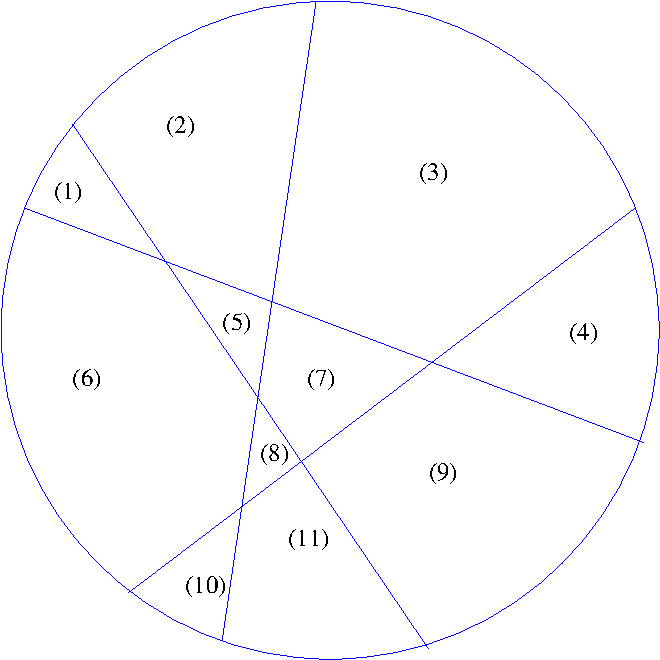
\includegraphics[scale=0.3]{graphics/pancakecut11}
			\captionsetup{labelformat=empty}
			\caption{}
			\label{fig:pancakecut11}
		\end{figure}
   
    \item AA\\
    
  \end{enumerate}
  \item $n = 4$\\
  \begin{enumerate}
    \item Pancake structure\\
      \begin{figure}[h!]
			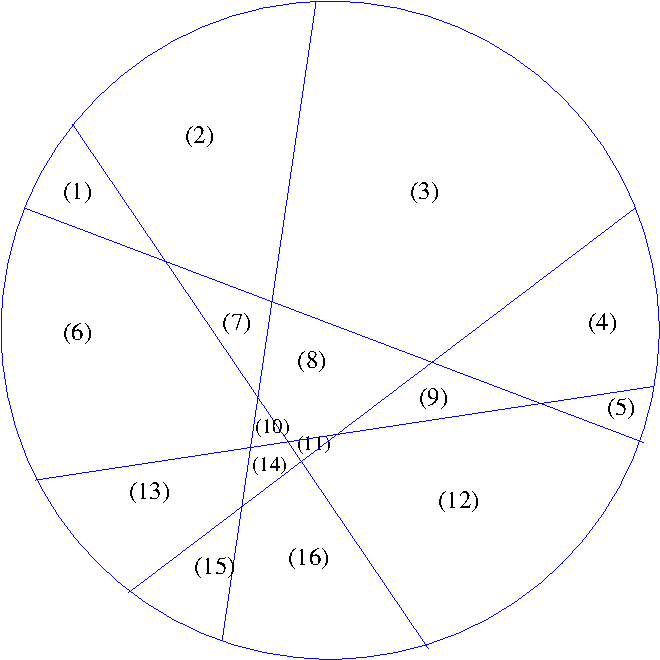
\includegraphics[scale=0.3]{graphics/pancakecut16}
			\captionsetup{labelformat=empty}
			\caption{}
			\label{fig:pancakecut16}
		\end{figure}
    \item AA\\
      
  \end{enumerate}
\end{enumerate}



\subsection{Formula Demonstrations}
	\begin{enumerate}
  \item $a(n) = Binomial(n+2,1)-2\times Binomial(n+1,1)+Binomial(n+2,2)$\\

  \hspace{1cm}${n+2 \choose 1} - 2\times {n+1 \choose 1} + {n+2 \choose 2}$\\
  \begin{enumerate}
    \item $n = 4$
    \[
     \boxed{ 
	  \begin{gathered}
       	a(4) = {4+2 \choose 1} - 2\times {4+1 \choose 1} + {4+2 \choose 2}\\
		\\ 
       	a(4) = {6 \choose 1} - 2\times {5 \choose 1} + {6 \choose 2} \\
       	\\
       	a(4) = 6 - 10 + 15\\
       	\\
       	a(4) = 11 
      \end{gathered}	    
	  }
    \]	  
    \item $ n = 5$
    \[
     \boxed{ 
	  \begin{gathered}
       	a(5) = {5+2 \choose 1} - 2\times {5+1 \choose 1} + {5+2 \choose 2}\\
		\\ 
       	a(5) = {7 \choose 1} - 2\times {6 \choose 1} + {7 \choose 2} \\
       	\\
       	a(5) = 7 - 12 + 21\\
       	\\
       	a(4) = 16 
      \end{gathered}	    
	  }
    \]	
  \end{enumerate}
  \item $G.f : A(x) = (1-x+x^2)/(1-x)^3$
  \begin{enumerate}
    \item $n = 4$
    \[
     \boxed{ 
	  \begin{gathered}
%       	a(4) = {4+2 \choose 1} - 2\times {4+1 \choose 1} + {4+2 \choose 2}\\
%		\\ 
%       	a(4) = {6 \choose 1} - 2\times {5 \choose 1} + {6 \choose 2} \\
%       	\\
%       	a(4) = 6 - 10 + 15\\
%       	\\
%       	a(4) = 11 
      \end{gathered}	    
	  }
    \]	  
    \item $ n = 5$
    \[
     \boxed{ 
	  \begin{gathered}
%       	a(5) = {5+2 \choose 1} - 2\times {5+1 \choose 1} + {5+2 \choose 2}\\
%		\\ 
%       	a(5) = {7 \choose 1} - 2\times {6 \choose 1} + {7 \choose 2} \\
%       	\\
%       	a(5) = 7 - 12 + 21\\
%       	\\
%       	a(4) = 16 
      \end{gathered}	    
	  }
    \]	
  \end{enumerate}
\end{enumerate} \fi
%end of commented out section

\end{document}
